\documentclass[11pt,a4paper]{article}

\usepackage[margin=1in]{geometry}
\usepackage{amsmath,amssymb}
\usepackage{booktabs}
\usepackage{graphicx}
\usepackage{xcolor}
\usepackage[numbers]{natbib}
\usepackage[colorlinks=true,linkcolor=blue!50!black,citecolor=blue!50!black,urlcolor=blue!50!black]{hyperref}



\title{\LARGE\textbf{Fine-Tuning CLIP for Remote-Sensing Image--Text Retrieval:}\\[4pt]
\large\textbf{Per-Scene Analysis and a Leakage-Aware Transfer Study}}
\author{Mohammed Abo Oraig \\ \small Independent research \\ \small \texttt{mohammed-abo-oraig@etud.univ-tln.fr}}
\date{}


\begin{document}
\maketitle

\begin{abstract}
We align remote-sensing images and captions in a shared embedding space by fine-tuning a pretrained CLIP dual encoder with a symmetric contrastive (InfoNCE) loss, and evaluate image-to-text and text-to-image retrieval. On a laptop GPU with 4~GB of memory, fine-tuning only the last transformer blocks raises the mean of the six Recall@$K$ scores on the RSICD test split from 15.5 (zero-shot CLIP) to $30.7\pm0.6$ (last 4 blocks) and $33.0\pm1.3$ (last 8 blocks), over three seeds. Every one of the 30 scene classes improves. On UCM-Captions, which the model never saw, mean recall rises by about 7 points over zero-shot CLIP, and adapting 8 instead of 4 blocks gives no additional benefit there. A near-duplicate analysis shows that 97.6\% of the RSITMD test images have a copy in RSICD, 80\% in its training or validation split, so a naive RSICD$\to$RSITMD transfer number would mostly measure memorized images; we report the 91 clean queries separately, where fine-tuning gains 16 to 19 points. We describe the protocol, the leakage check, and the limits of this small study.
\end{abstract}

\section{Introduction}
Cross-modal retrieval asks for the images that match a text query and the texts that describe a query image. General-purpose contrastive models such as CLIP \citep{radford2021clip} are trained on web images; aerial scenes are a different visual domain, with top-down viewpoints, no canonical orientation, and many visually similar classes (residential densities, farmland versus bareland). Remote-sensing-specific models trained on large collections of aerial image--text pairs exist \citep{liu2024remoteclip}. Here we ask a smaller, practical question: how far can a pretrained CLIP be adapted on a single public dataset, with modest hardware, and how well does the adaptation generalize? We study three questions:
\begin{enumerate}
  \item[\textbf{Q1}] How much does contrastive fine-tuning improve retrieval in both directions, and how many layers need to be adapted?
  \item[\textbf{Q2}] How does the improvement vary across scene classes?
  \item[\textbf{Q3}] Does it transfer to datasets the model was not trained on?
\end{enumerate}
Answering Q3 turned out to require care: the two public benchmarks we tried for transfer behave very differently with respect to overlap with the training data (Section~\ref{sec:overlap}). Code is available at \url{https://github.com/AboOraig/vl-retrieval}.

\section{Data}
\paragraph{RSICD} \citep{lu2018rsicd} has 10{,}921 aerial images (224$\times$224 pixels) with five captions each, in 30 scene classes; we use the official split (8{,}734 train, 1{,}094 validation, 1{,}093 test). The class is encoded in the file name for 10{,}000 images; the other 921 have numbered file names without a label. These are used everywhere except in the per-class analysis.
\paragraph{UCM-Captions} \citep{qu2016ucm} has 2{,}100 images with five captions each (1{,}680 / 210 / 210). File names carry no class label.
\paragraph{RSITMD} \citep{yuan2022rsitmd} has 4{,}743 images with five fine-grained captions each (4{,}291 train, 452 test, no validation split) and class-bearing file names.
Training uses RSICD only. UCM-Captions and RSITMD are used only for evaluation, with their official test splits.

\section{Method}
\paragraph{Model.} A dual encoder: OpenCLIP \citep{ilharco2021openclip} ViT-B/32 initialised from the OpenAI weights \citep{radford2021clip} (151M parameters), producing $\ell_2$-normalised image and text embeddings $f(x),g(t)$. (The OpenAI weights must be loaded into the QuickGELU variant of the architecture; the plain variant silently degrades the embeddings.)
\paragraph{Loss.} For a batch of $B$ pairs $(x_i,t_i)$ with similarities $s_{ij}=\cos(f(x_i),g(t_j))$ and temperature $\tau$,
\begin{equation}
\mathcal L=\tfrac12\Big[-\tfrac1B\sum_i\log\frac{e^{s_{ii}/\tau}}{\sum_j e^{s_{ij}/\tau}}-\tfrac1B\sum_i\log\frac{e^{s_{ii}/\tau}}{\sum_j e^{s_{ji}/\tau}}\Big],
\end{equation}
the symmetric InfoNCE loss \citep{oord2018cpc,radford2021clip}, with $1/\tau$ a learned parameter clamped at $100$. In practice it stayed at its pretrained value of about 100 throughout training.
\paragraph{Batches.} Each epoch visits every training image once, with one of its five captions drawn at random. A batch therefore contains $B=64$ distinct images, so no other caption in the batch is a hidden positive for an image.
\paragraph{Which layers are trained.} Three variants, all starting from the pretrained weights: (i) the two projection layers, the final layer norms and the temperature (0.7M parameters); (ii) additionally the last 4 transformer blocks of both towers (41.6M); (iii) the last 8 blocks (82.6M). Fine-tuning every layer did not fit in 4~GB of GPU memory and was not run.
\paragraph{Optimization.} AdamW \citep{loshchilov2019adamw} with learning rate $10^{-5}$ and weight decay $0.1$ (not applied to biases, norms or the temperature), 5\% linear warm-up followed by cosine decay \citep{loshchilov2017sgdr}, gradient-norm clipping at 1.0, fp16 mixed precision \citep{micikevicius2018mixed}, random horizontal/vertical flips and 90$^\circ$ rotations of the image, at most 15 epochs. After each epoch the mean recall on the validation split is computed; training stops after four epochs without improvement, and the best epoch is kept. The test split is evaluated once, with that checkpoint. No hyperparameter other than the number of trained layers was varied.

\section{Evaluation protocol}
Retrieval is evaluated within one split: every image is a query against all captions of the split (image-to-text, i2t), and every caption is a query against all images (text-to-image, t2i). A caption query is correct if its image is in the top $K$; an image query is correct if \emph{any} of its five captions is in the top $K$. We report Recall@1/5/10 in both directions and \emph{mR}, the mean of the six values. Ties are counted against the model. Results are mean $\pm$ sample standard deviation over three training seeds, except for zero-shot CLIP (deterministic) and the projection-only variant (one run). Gallery sizes differ between datasets (1{,}093, 210 and 452 images), and recall grows as the gallery shrinks, so absolute scores are comparable between methods on one dataset but not between datasets.

\paragraph{Overlap check.}\label{sec:overlapmethod} To test whether an evaluation set shares images with the training data, each image is reduced to a 256-bit difference hash (grayscale, resized to $17\times16$, sign of horizontal gradients) that is robust to re-encoding and rescaling; each query image is compared in its 8 rotations and reflections with every RSICD image, and the closest pair is also inspected visually. Pairs within 20 bits are treated as duplicates.

\section{Results}
\subsection{In-domain retrieval on RSICD}
\begin{table}[t]
\centering\small
\caption{RSICD test split (1{,}093 images, 5{,}465 captions). Recall in \%. Mean $\pm$ sd over three seeds where indicated.}\label{tab:rsicd}
\resizebox{\textwidth}{!}{%
\begin{tabular}{lccccccccc}
\toprule
 & & \multicolumn{3}{c}{image$\to$text} & \multicolumn{3}{c}{text$\to$image} & \\
\cmidrule(lr){3-5}\cmidrule(lr){6-8}
Method & Runs & R@1 & R@5 & R@10 & R@1 & R@5 & R@10 & mR \\
\midrule
Zero-shot CLIP & 1 & 4.9 & 14.4 & 23.0 & 5.5 & 17.6 & 27.8 & 15.5 \\
Projections only & 1 & 8.5 & 22.7 & 34.4 & 7.9 & 26.4 & 41.1 & 23.5 \\
Last 4 blocks & 3 & \pmsd{13.0}{0.7} & \pmsd{30.8}{1.3} & \pmsd{44.8}{1.7} & \pmsd{12.1}{0.5} & \pmsd{33.2}{0.2} & \pmsd{50.1}{0.9} & \pmsd{30.7}{0.6} \\
Last 8 blocks & 3 & \pmsd{16.0}{1.0} & \pmsd{33.5}{2.7} & \pmsd{45.9}{1.9} & \pmsd{13.0}{0.6} & \pmsd{36.6}{1.0} & \pmsd{53.2}{1.1} & \pmsd{\textbf{33.0}}{1.3} \\
\bottomrule
\end{tabular}}
\end{table}
Fine-tuning roughly doubles mean recall and triples image-to-text R@1 (Table~\ref{tab:rsicd}). More trainable layers help, with diminishing returns: the increments in mR are about $+8$ (projections), $+7.2$ (4 blocks) and $+2.3$ (8 blocks) over the previous row. The seed-to-seed standard deviation is 0.6 for 4 blocks and 1.3 for 8 blocks, so the last increment is modest relative to the variation. Retrieval in the text-to-image direction is better at $K=10$ and the image-to-text direction at $K=1$ for the fine-tuned models. For context, RemoteCLIP \citep{liu2024remoteclip} reports 35.3 mR on RSICD for the same backbone, using substantially more remote-sensing training data and its own protocol; we did not re-run it and draw no ranking.

\subsection{Per scene class}
\begin{figure}[hpt]
\centering
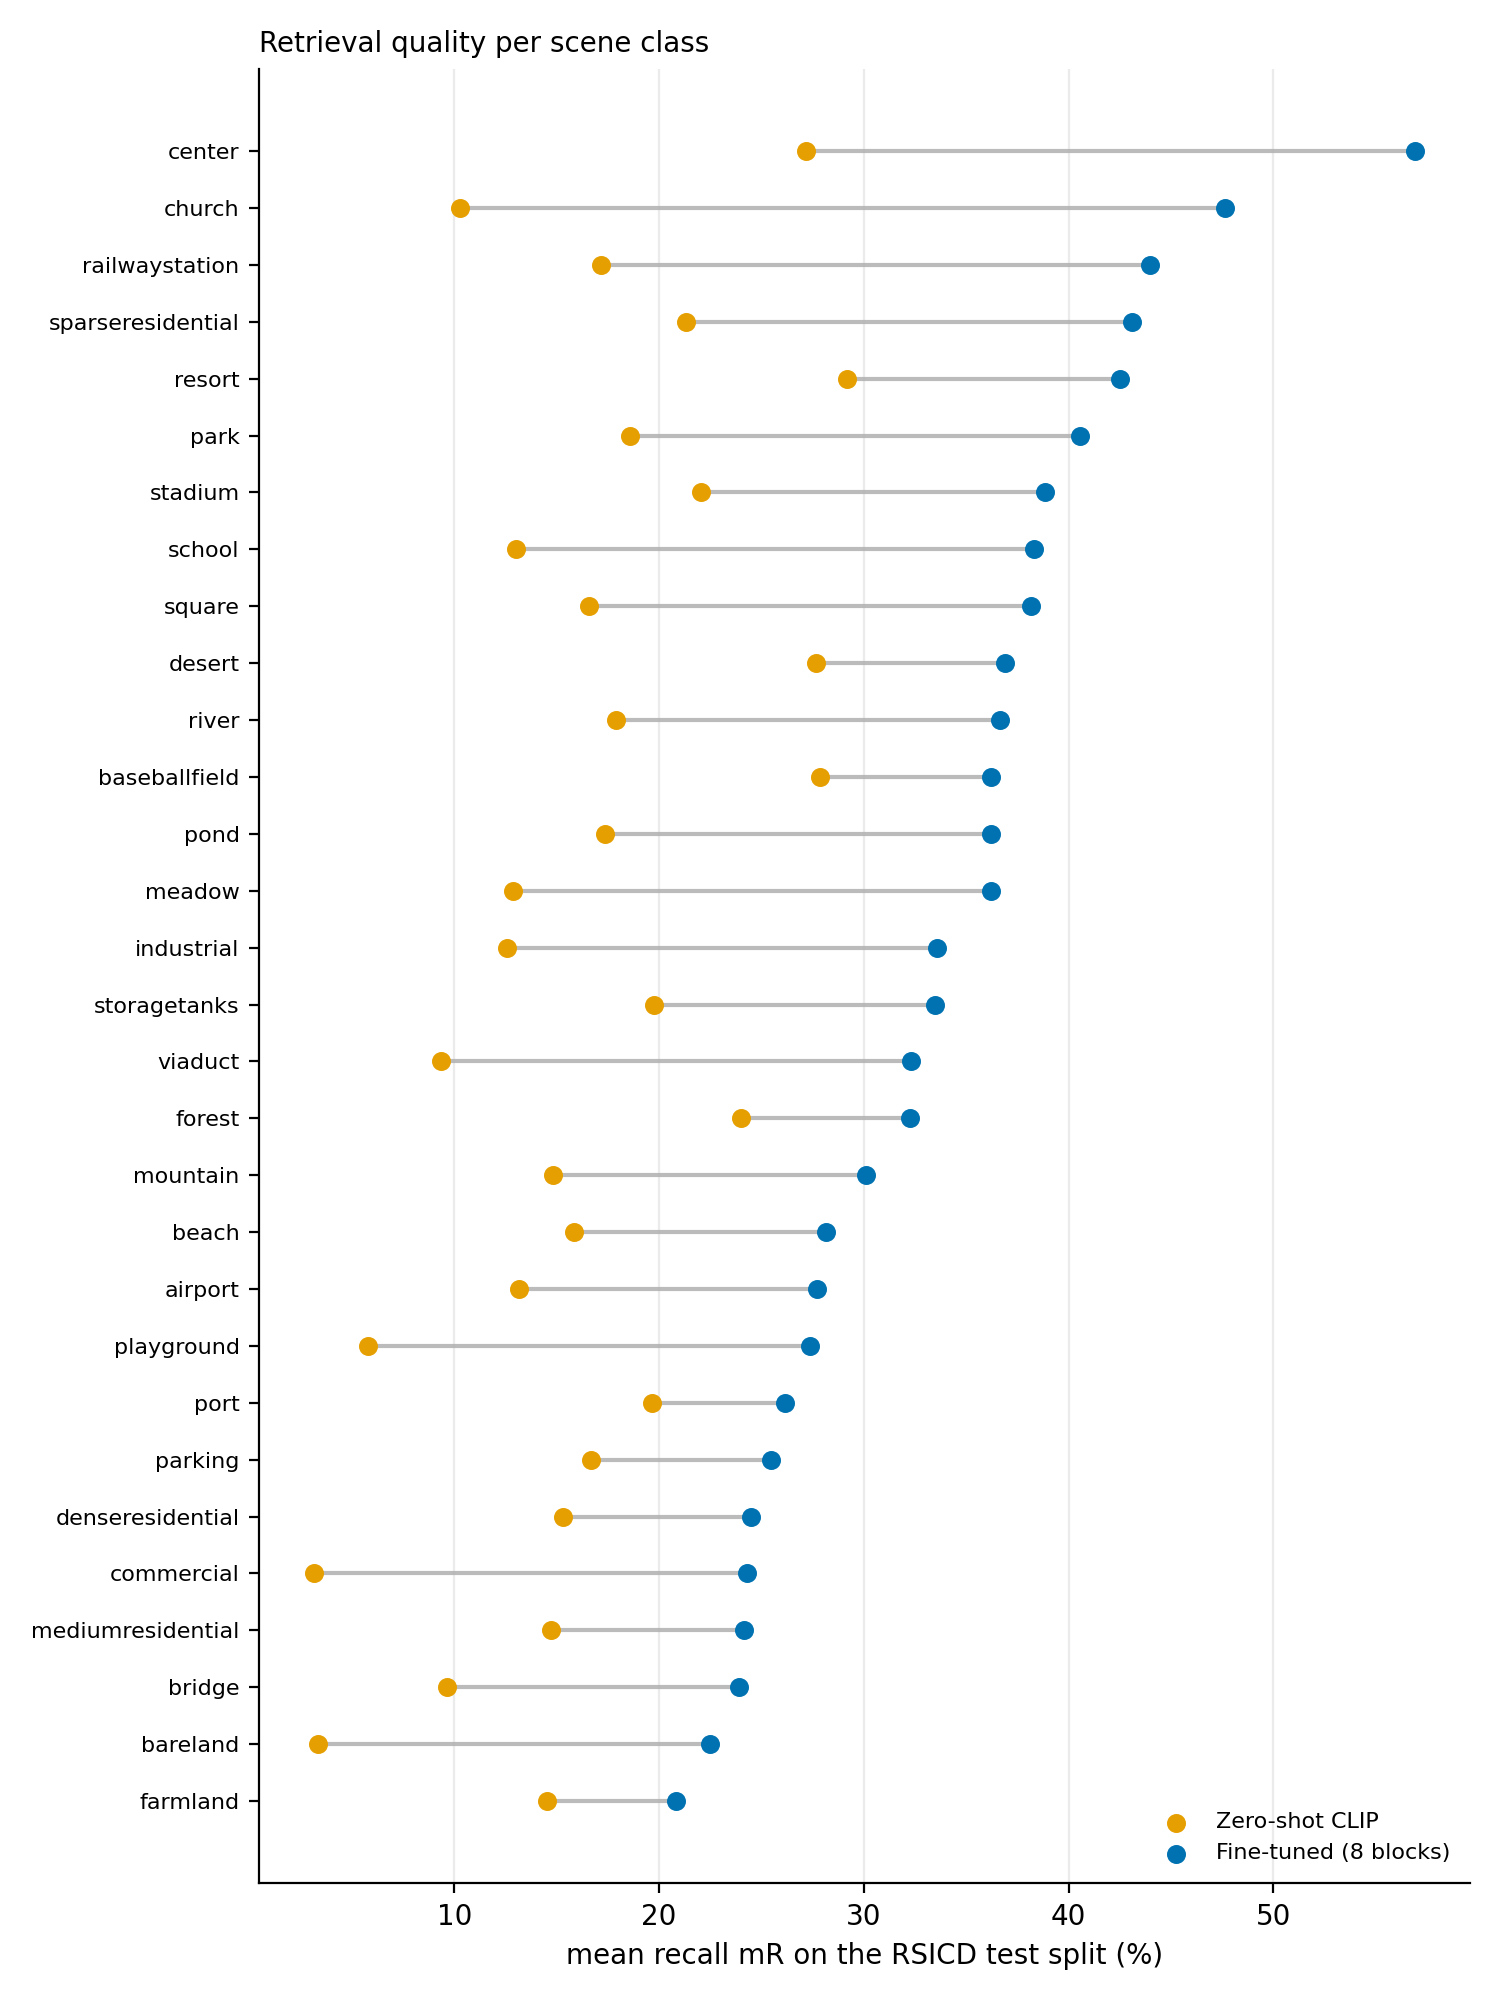
\includegraphics[width=0.78\textwidth]{figures/per_scene.png}
\caption{Mean recall per RSICD scene class on the test split, zero-shot CLIP versus the 8-block model (seed 0). Each class has 24--46 query images; 66 test images without a class label are excluded as queries but remain in the gallery.}\label{fig:perscene}
\end{figure}
Fine-tuning improves all 30 classes, by $+6.3$ to $+37.4$ mean-recall points (Figure~\ref{fig:perscene}). The largest gains are for church ($+37.4$), center ($+29.7$), railway station ($+26.8$) and school ($+25.3$), the smallest for farmland ($+6.3$), port ($+6.5$), forest and baseball field ($+8.3$). After fine-tuning the best classes are center (56.9), church (47.6) and railway station (44.0), the worst farmland (20.8), bareland (22.5) and bridge (23.9). A plausible reading, which we did not test, is that classes defined by a distinctive structure are learned quickly, whereas visually homogeneous classes (farmland, bareland) and classes with close neighbours (dense, medium and sparse residential; commercial) remain hard because many gallery images and captions look alike. With 24--46 queries per class, differences of a few points between classes are within noise.

\subsection{Transfer to UCM-Captions}
\begin{table}[t]
\centering\small
\caption{UCM-Captions test split (210 images, 1{,}050 captions), models trained on RSICD only. Recall in \%.}\label{tab:ucm}
\resizebox{\textwidth}{!}{%
\begin{tabular}{lccccccccc}
\toprule
 & & \multicolumn{3}{c}{image$\to$text} & \multicolumn{3}{c}{text$\to$image} & \\
\cmidrule(lr){3-5}\cmidrule(lr){6-8}
Method & Runs & R@1 & R@5 & R@10 & R@1 & R@5 & R@10 & mR \\
\midrule
Zero-shot CLIP & 1 & 6.2 & 22.9 & 46.7 & 8.7 & 36.4 & 60.3 & 30.2 \\
Projections only & 1 & 6.7 & 21.9 & 53.3 & 10.8 & 43.1 & 72.5 & 34.7 \\
Last 4 blocks & 3 & \pmsd{8.9}{0.3} & \pmsd{24.0}{0.3} & \pmsd{58.6}{2.9} & \pmsd{12.8}{0.7} & \pmsd{47.1}{0.4} & \pmsd{75.0}{0.8} & \pmsd{37.7}{0.6} \\
Last 8 blocks & 3 & \pmsd{8.4}{1.8} & \pmsd{24.4}{2.4} & \pmsd{56.8}{3.3} & \pmsd{13.5}{0.8} & \pmsd{47.0}{1.8} & \pmsd{74.6}{2.4} & \pmsd{37.5}{1.2} \\
\bottomrule
\end{tabular}}
\end{table}
No UCM test image is close to any RSICD image (distance to the closest RSICD image: minimum 35 bits, median 87; Section~\ref{sec:overlap}), so this is a genuine transfer test. Training on RSICD raises mean recall on UCM by about 7 points over zero-shot CLIP (Table~\ref{tab:ucm}) in both directions. Unlike on RSICD, adapting 8 blocks is no better than 4 here ($37.5\pm1.2$ versus $37.7\pm0.6$): the additional capacity helps in-domain but does not buy additional transfer.

\subsection{RSITMD and the overlap with RSICD}\label{sec:overlap}
Of the 452 RSITMD test images, 441 (97.6\%) have a near-duplicate among the RSICD images; the median distance to the closest RSICD image is 6 bits, against 87 bits for UCM (Section~\ref{sec:overlapmethod}), and the closest pairs are visibly the same photographs. For 361 images (80\%) the copy lies in RSICD's training or validation split. Training on RSICD and testing on RSITMD would therefore mostly evaluate images seen in training. We split the RSITMD queries into the 91 images with no copy in RSICD's training or validation split, which form a valid transfer test, and the 361 with one, always ranking against the full 452-image gallery (Table~\ref{tab:rsitmd}).
\begin{table}[t]
\centering\small
\caption{RSITMD test split (452 images), models trained on RSICD only: mR, by whether the query image also occurs in RSICD's training or validation split.}\label{tab:rsitmd}
\begin{tabular}{lcccc}
\toprule
Method & Runs & 91 clean queries & 361 queries seen in RSICD & all 452 \\
\midrule
Zero-shot CLIP & 1 & 29.6 & 22.8 & 24.2 \\
Projections only & 1 & 39.2 & 36.3 & 36.9 \\
Last 4 blocks & 3 & \pmsd{45.5}{1.6} & \pmsd{50.8}{5.5} & \pmsd{49.7}{4.7} \\
Last 8 blocks & 3 & \pmsd{48.4}{1.9} & \pmsd{55.4}{7.9} & \pmsd{54.0}{6.5} \\
\bottomrule
\end{tabular}
\end{table}
On clean queries, fine-tuning on RSICD improves mean recall by 16 (4 blocks) to 19 (8 blocks) points over zero-shot CLIP, and the 8-block model is ahead of the 4-block one by about 3 points, a difference of roughly the size of the seed variation. On the seen queries the improvement is larger ($+28$ to $+33$) and the seed-to-seed spread much larger (5.5 to 7.9), which is consistent with a benefit from training images; however the two groups also differ in content, so this is not a controlled comparison. The clean group has only 91 queries.

\section{Discussion and limitations}
\paragraph{What the results support.} Contrastive fine-tuning of a pretrained dual encoder roughly doubles retrieval quality on RSICD, improves every scene class, and the gain carries over to data from other sources that the model has never seen. Adapting more layers helps in-domain but, on UCM, not out of domain.
\paragraph{Lessons on evaluation.} The RSITMD overlap shows that two public benchmarks can share imagery without this being obvious from their documentation; a transfer number between them is uninterpretable without such a check. Inspecting the closest pairs was as informative as the hash distances.
\paragraph{Limitations.} Training uses one dataset; one hyperparameter setting (learning rate, batch size, augmentation) was used and not tuned. Zero-shot and projection-only numbers are single runs; three seeds give only a rough estimate of variation. The test sets are small (452 and 210 images), the per-class results rest on 24--46 queries and the RSITMD clean group on 91, and gallery sizes differ between datasets, so absolute scores are not comparable across tables. The epoch is selected on a 1{,}094-image validation split, which is noisy (the 4-block model stopped at epoch 3 for one seed and at epoch 7 for another). Captions are truncated to CLIP's 77 tokens. Full fine-tuning, larger backbones and training on several datasets were not tried; the comparison with RemoteCLIP is context, not a benchmark. Software and hardware: PyTorch \citep{paszke2019pytorch} 2.5.1 (CUDA 12.1), Python 3.11, OpenCLIP 4.2.2; an RTX~3050 laptop GPU with 4~GB (peak memory 1.4, 2.1 and 3.5~GiB for the three variants; roughly 9, 6--13 and 25 minutes per run).

\section{Conclusion}
Fine-tuning the last transformer blocks of a pretrained CLIP with a symmetric contrastive loss improves remote-sensing image--text retrieval in both directions, from 15.5 to $33.0\pm1.3$ mean recall on RSICD, for every scene class, and by about 7 points zero-shot on UCM-Captions. A near-duplicate check, which should accompany any RSICD/RSITMD transfer experiment, shows that most of the RSITMD test set is contained in RSICD; on the 91 clean queries the improvement remains, at 16 to 19 points.

\bibliographystyle{plainnat}
\bibliography{references}
\end{document}
